\section{Empirical Results}
\label{sec:results}

The controlled comparisons in Section~\ref{subsec:evaluation_design} address four related questions. E1 tests whether delay-based priorities retain the consequence-based screening shortlist and whether passenger or downstream exposure improves the screening decision. E2 compares temporal and probabilistic information representations across screening and local-recovery decisions. E3 examines how the value of joint-state dependence varies across the four prespecified objective-weight settings. E4 describes annual and PRE/TURN heterogeneity in these relationships. We report the screening comparison first, then characterize recoverable value within the annual History+Joint (HJ) reference cohorts, compare information representations across the two decision layers, and assess objective sensitivity. The annual support populations and evaluation protocol are summarized in Section~\ref{subsubsec:temporal_design}. The available results use prespecified canonical decision epochs; they do not provide within-chain rolling-epoch trajectories.

\subsection{Delay-based Screening under a Fixed Review Budget}
\label{subsec:results_screening}

E1 asks whether expected delay alone is an adequate priority when only a fixed share of flight chains can receive detailed review. At the nominal review share $q_0=0.10$, the Delay priority replaces 37--53\% of PRE shortlist positions and 40--55\% of TURN positions relative to the consequence-based reference. These replacements carry normalized reference-consequence losses $L^{\mathrm{att}}=0.101$--$0.184$ in PRE and $0.107$--$0.181$ in TURN. The losses are positive in every annual stage-specific comparison, showing that expected delay does not preserve the consequence-based shortlist at the active review boundary.

\begin{figure}[pos=t]
\centering
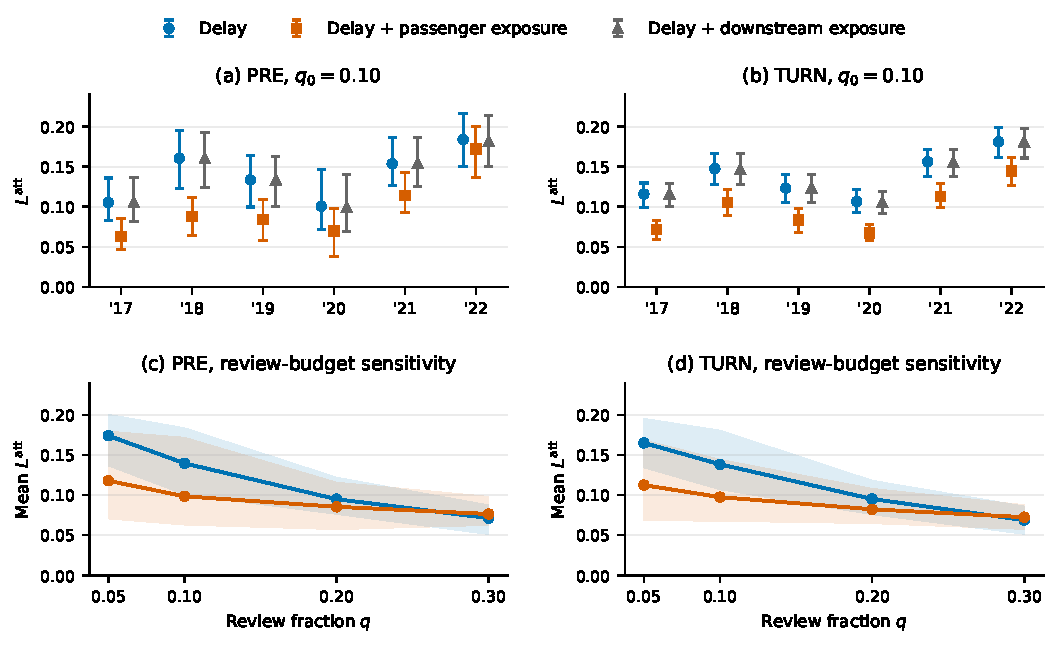
\includegraphics[width=0.99\linewidth]{figures/figure_s5_1_q_boundary.pdf}
\caption{Delay-only screening loses reference consequence under the nominal review budget, while passenger exposure recovers part of that loss. Panels~(a)--(b) show annual PRE and TURN $L^{\mathrm{att}}$ estimates at $q_0=0.10$ with episode-cluster percentile-bootstrap 95\% intervals for each priority. Panels~(c)--(d) show the mean $L^{\mathrm{att}}$ across years over the review-budget grid; shaded bands give the annual minimum-to-maximum range, not confidence intervals.}
\label{fig:q_boundary}
\end{figure}

The intermediate Delay+Passenger priority reduces the Delay screening loss by 6--45\% in PRE and 20--38\% in TURN, but a substantial gap from the consequence reference remains in all year-stage settings. The Delay+Downstream priority behaves differently: its shortlist and $L^{\mathrm{att}}$ remain close to those of Delay, with an absolute loss difference no greater than 0.003 in any of the twelve year-stage comparisons. Thus, the observed incremental screening value is associated primarily with passenger exposure in this evaluation, although that signal does not fully recover the consequence-based ranking.

The review-budget analysis qualifies this result. As $q$ increases from 0.05 to 0.30, the year-mean Delay loss falls from 0.174 to 0.071 in PRE and from 0.165 to 0.069 in TURN. At $q=0.30$, the mean loss gap between Delay and Delay+Passenger is at most 0.006 in either stage. The disagreement is therefore most consequential when detailed review capacity is tight; larger review budgets reduce, but do not redefine, the difference between delay and consequence priorities.

\subsection{Recoverable Value in the HJ Reference Cohorts}
\label{subsec:results_local_recovery}

The E2 local-recovery analysis uses the annual HJ consequence-based shortlist intersected with valid Stage-II support. This cohort describes the recoverable value among cases selected for reference review; it does not represent the full Stage-II-eligible population. Table~\ref{tab:stage2_recovery_profile} summarizes its Balanced-objective profile across the six years.

\begin{table}[pos=t]
\centering
\caption{Balanced-objective recoverable value within annual HJ reference cohorts.}
\label{tab:stage2_recovery_profile}
\small
\setlength{\tabcolsep}{5pt}
\begin{tabular}{lrrrrr}
\toprule
Year & $N$ & $\Pr(u^*>0)$ & Median $V^{HJ}$ (CU) & P90 $V^{HJ}$ (CU) & $\sum_i V_i^{HJ}$ (CU) \\
\midrule
2017 & 521 & 0.843 & 0.018 & 0.236 & 40.4 \\
2018 & 523 & 0.906 & 0.136 & 0.360 & 85.1 \\
2019 & 515 & 0.823 & 0.023 & 0.242 & 42.1 \\
2020 & 474 & 0.916 & 0.055 & 0.201 & 41.4 \\
2021 & 523 & 0.885 & 0.111 & 0.249 & 65.4 \\
2022 & 532 & 0.902 & 0.124 & 0.333 & 78.3 \\
\bottomrule
\end{tabular}
\par\vspace{3pt}
\begin{minipage}{0.98\linewidth}
\footnotesize
$N$ is the annual HJ reference-cohort size. $V_i^{HJ}=J_i^{HJ}(0)-J_i^{HJ}(u_i^*)$ is model-recoverable value under the Balanced objective. CU denotes the normalized consequence unit; these quantities are model-based and are not observed monetary savings. Stage-specific support counts are reported in Table~\ref{tab:annual_evaluation_support}.
\end{minipage}
\end{table}

Across the annual reference cohorts, the HJ target is positive for 82--92\% of cases. The median per-case recoverable value ranges from 0.018 CU in 2017 to 0.136 CU in 2018, while the P90 ranges from 0.201 to 0.360 CU. The annual sum of reference recoverable value ranges from 40.4 to 85.1 CU. Activation is higher in TURN than PRE in every year (0.83--0.93 versus 0.77--0.88), consistent with the lower zero-value share in TURN (0.074--0.175) than PRE (0.115--0.229).

These quantities distinguish baseline consequence from remaining local-recovery opportunity, but they do not establish how recoverable value is distributed over the full eligible population or whether a particular screening rule captures more of that value. Recovery-opportunity Coverage@K and the priority--recoverability association over the full eligible set are not reported because the current held-out outputs provide recoverable values for the annual reference cohorts only.

\subsection{Information Effects across Screening and Local Recovery}
\label{subsec:results_information}

E2 compares History+Marginal (HM) and History+Point (HP) with History+Joint (HJ) on paired common-support populations. The Stage-I and Stage-II outcomes have different reference objects, so their losses are reported separately and are not interpreted as a common performance scale. Table~\ref{tab:information_decision_summary} summarizes the six-year ranges; Figure~\ref{fig:information_layers} shows the annual estimates. Full annual contrast rows and interval estimates appear in Supplementary Table~\ref{tab:sup_e2_support_detail}.

\begin{table}[pos=t]
\centering
\caption{Six-year ranges of direct paired contrasts between information representations.}
\label{tab:information_decision_summary}
\small
\setlength{\tabcolsep}{4pt}
\begin{tabular}{lrrrr}
\toprule
Contrast & Stage-I positions reassigned & $L^{\mathrm{att}}$ & Stage-II $A_0$ & $L^{\mathrm{rec}}$ \\
\midrule
HM--HJ & 1.3--3.8\% & 0.0006--0.0026 & 0.581--0.730 & 0.0853--0.1247 \\
HP--HJ & 84.2--88.7\% & 0.4134--0.5291 & 0.130--0.241 & 0.8963--0.9814 \\
\bottomrule
\end{tabular}
\par\vspace{3pt}
\begin{minipage}{0.98\linewidth}
\footnotesize
Entries are the minimum-to-maximum annual point estimates across 2017--2022. The Stage-I and Stage-II losses use distinct reference quantities. The table reports direct contrasts against HJ; the separate paired HP--HM loss increment is described in the text below.
\end{minipage}
\end{table}

Replacing the Joint coupling with the weighted-Marginal coupling changes only a small share of the screening shortlist: HM--HJ reassigns 1.3--3.8\% of positions and has $L^{\mathrm{att}}=0.0006$--$0.0026$, retaining more than 99.6\% of the reference shortlist consequence. The local-recovery result is less stable. Exact target agreement is $A_0=0.581$--$0.730$, and the normalized reference loss is $L^{\mathrm{rec}}=0.085$--$0.125$. Near-identical screening shortlists therefore do not imply identical local-recovery targets.

The Point representation produces a larger loss relative to HJ at both decision layers. HP--HJ reassigns 84.2--88.7\% of shortlist positions, with $L^{\mathrm{att}}=0.4134$--$0.5291$; Stage-II exact target agreement falls to $A_0=0.130$--$0.241$, and $L^{\mathrm{rec}}=0.8963$--$0.9814$. The paired HP--HM loss increment is $0.4095$--$0.5291$ for Stage-I $L^{\mathrm{att}}$ and $0.8040$--$0.8879$ for Stage-II $L^{\mathrm{rec}}$. These estimates use their own paired common-support samples and are not arithmetic differences between the HP--HJ and HM--HJ rows in Table~\ref{tab:information_decision_summary}; shortlist reassignment and $A_0$ are not defined for this loss-increment contrast. Within the tested consequence model and supported cohorts, compressing the state distribution to a point therefore changes decisions more than replacing joint dependence while retaining the weighted primitive marginals. The paired increment is not an additive decomposition of HP--HJ loss.

The component audit provides a model-specific explanation for the comparatively small HM--HJ loss. Under the validated weighted-Marginal coupling, Flight and Resource domain scores match their Joint counterparts to numerical precision for all audited candidates (maximum absolute difference below $10^{-13}$ CU). The Passenger domain differs for 39--66\% of candidates through threshold-event exposure, whose probability can depend on cross-state coupling. Dependence thus affects the current recovery criterion through its nonseparable threshold consequences; this finding is specific to the stated consequence construction.

\begin{figure}[pos=t]
\centering
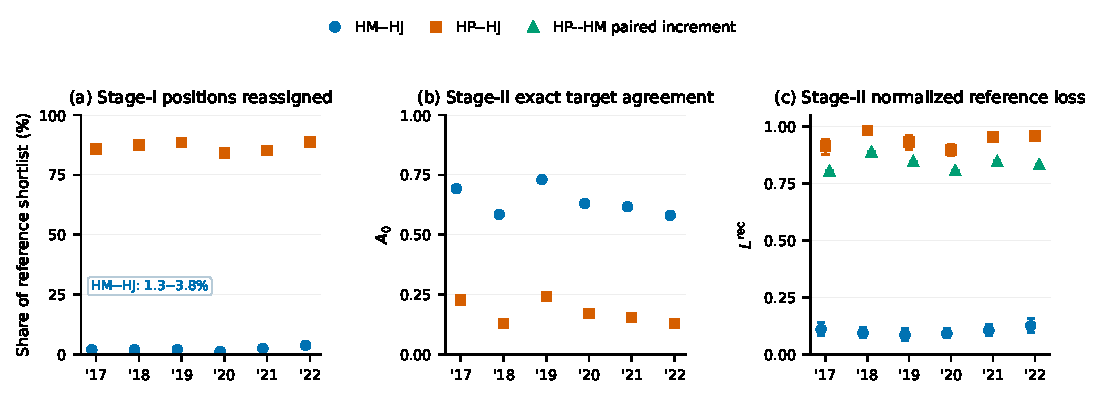
\includegraphics[width=0.99\linewidth]{figures/figure_s5_2_information_layers_v2.pdf}
\caption{Information compression has sharply different effects on screening and local-recovery decisions. Panel~(a) reports the share of reference shortlist positions reassigned under HM--HJ and HP--HJ. Panel~(b) reports Stage-II exact target agreement $A_0$ for HM--HJ and HP--HJ. Panel~(c) reports Stage-II $L^{\mathrm{rec}}$ for HM--HJ, HP--HJ, and the paired HP--HM Point-minus-Marginal increment, with episode-cluster percentile-bootstrap 95\% intervals. The paired increment is estimated on its own common-support population and is not an arithmetic decomposition of the other contrasts.}
\label{fig:information_layers}
\end{figure}

\subsection{Objective Sensitivity and Annual--Stage Heterogeneity}
\label{subsec:results_objectives}
\label{subsec:results_heterogeneity}

E3 recomputes the Marginal and Joint targets under four prespecified objective-weight settings, evaluating each decision against the Joint reference for that objective. Exact HM--HJ target agreement ranges from 0.581--0.730 under Balanced, 0.593--0.739 under Flight emphasis, 0.547--0.664 under Passenger emphasis, and 0.608--0.772 under Resource emphasis. Passenger emphasis has the lowest agreement in all six years, while Resource emphasis has the lowest activation share (0.631--0.835) and the largest zero-recoverable-value share (0.165--0.369). These comparisons show that the observed decision sensitivity depends on the chosen objective; no single objective yields a year-invariant agreement level.

The objective comparison also reveals a mass-at-zero pattern obscured by the mean alone. The median absolute target change is zero in all 24 year-objective settings, although the mean ranges from 1.8 to 4.7 minutes and the maximum change in each setting lies between 30 and 45 minutes. Figure~\ref{fig:objective_dependence} separates exact target agreement from the mean target shift conditional on a change. This presentation shows both how often dependence leaves the selected target unchanged and the magnitude of the shift when it does change.

\begin{figure}[pos=t]
\centering
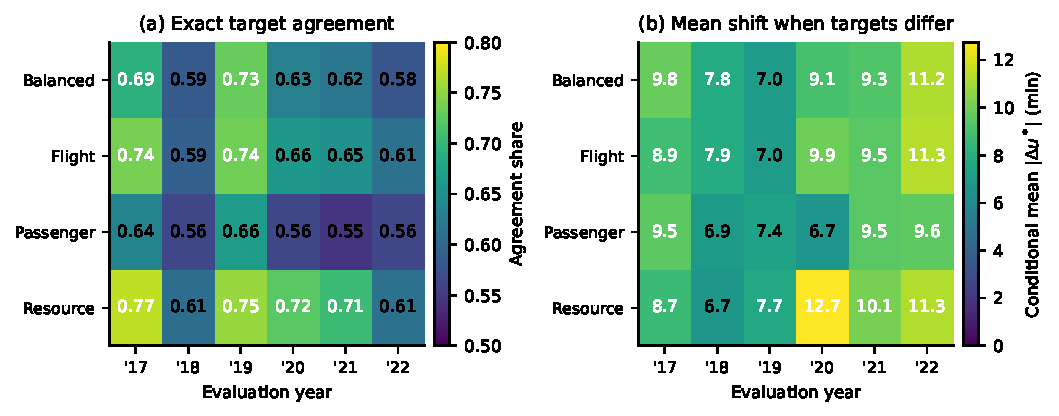
\includegraphics[width=0.99\linewidth]{figures/figure_s5_3_objectives.pdf}
\caption{Objective-specific target changes combine a substantial mass of unchanged choices with larger shifts among changed cases. Panel~(a) reports annual exact HM--HJ target agreement. Panel~(b) reports the mean absolute target change conditional on disagreement, calculated as the unconditional mean absolute change divided by the disagreement share. The 24 cells use the same annual HJ reference cohorts; no confidence intervals are shown.}
\label{fig:objective_dependence}
\end{figure}

Annual and stage-specific estimates are presented throughout rather than pooled into broad operating-period categories. The secondary Current--History comparison is year-dependent: across 2017--2022, $L^{\mathrm{att}}$ ranges from 0.010 to 0.506, $A_0$ from 0.086 to 0.495, and $L^{\mathrm{rec}}$ from 0.310 to 0.998. This remains an implemented-configuration contrast and does not isolate a causal effect of historical information. The current canonical-epoch outputs also do not identify within-chain trajectories or the threshold-by-headroom ablation; no results for those analyses are inferred here.

Across the six annual evaluations, the evidence supports two distinct decision-level findings. Marginal preservation is nearly sufficient for the fixed-capacity screening shortlist but not for exact local-recovery targeting. By contrast, point-value compression produces large losses at both layers, with a substantially larger paired increment than the dependence-only contrast. Objective-specific agreement and the distribution of target changes qualify this ordering and show why a single aggregate score would hide meaningful decision heterogeneity.
